\cotefile{84}
\scanpage{178}

Compatibilités pour

\diagram{\begin{tikzcd}[ampersand replacement=\&,column sep=small]
 A_1,A_2 \arrow[r,shift left=.5ex]\arrow[r,shift right=.5ex] \& A_1\otimes_0 A_2 \arrow[r,"\overline{\mathrm{Tr}}"]\arrow[dr,hook] \& O\arrow[dr] \& {}\\
 {} \& {} \& A_1\otimes A_2 \arrow[r,no head] \& A
\end{tikzcd}}

\diagram{\begin{tikzcd}[ampersand replacement=\&,column sep=small]
 E_1\otimes L_2,L_1\otimes A_2\arrow[r,shift left=.5ex]\arrow[r,shift right=.5ex] \& E_1\otimes_0 E_2\arrow[r,two heads,"\pi"]\arrow[dr,hook] \& L_1\otimes L_2\arrow[dr]\arrow[r] \& \deleted{\unsure{\longleftarrow|\longrightarrow}}\\
 {} \& {} \& E_1\otimes E_2\arrow[r] \& E
\end{tikzcd}}

Il y a à écrire quatre compatibilités.

$1^\circ)$ si $u\in L_1\otimes L_2$, $x\in E_1\otimes E_2$, alors $u\oplus x$ donne \deleted{\unsure{même chose pour|donc pour}} $\underline{O}\oplus(A_1\otimes A_2)\longrightarrow\underline{O}$ qui donne \unsure{même|$=$} chose sur $A_1$.

$2^\circ)$ $\deleted{\unsure{x}}f\in A_1\otimes_0 A_2$ alors $\langle\underbrace{f+f^{\unsure{t|tr|\sigma}}}_{\mathrm{Tr}f.1},\deleted{\unsure{f}}x\rangle=\mathrm{Tr}f\langle1\otimes1,x\rangle$

$3^\circ)$ $\unsure{x|t}\in E_1\otimes E_2\qquad \langle f,x+\overline{x}\rangle=\langle f,\pi(x)\rangle={\varphi}f.\pi(x)$

\noindent\rule{.20\linewidth}{.4pt}\par
OK \hspace{6em}$\unsure{=|t}$\par
\hspace{9em}\unsure{un}\par
\noindent\rule{.85\linewidth}{.4pt}

% archive sheet number: 177
\scanpage{179}
\mspage{493}

s c e n c e (*) d e \ l ' a u t r e \ t e r m e, constitue un état de déséquilibre grave, et à la limite (quand ``l'absence'' en question est quasiment complète, et prolongée) un état qui mène à la destruction de la chose (ou de l'être\unsure{)|:} en laquelle ce déséquilibre a lieu, voire même de lui et de son entourage.

Ainsi, un état d' a c t i o n ininterrompue, qui n'alterne avec des périodes suffisantes d' i n a c t i o n , de repos, mène à l'épuisement, la maladie et (à la limite) à la mort - chose d'ailleurs qui a été des plus actuelles dernièrement, pour moi! (**) Mais inversement, un état d'inaction excessif mène à un affaiblissement et à une sclérose des capacités et fonctions du corps ou du psychisme (suivant les cas), et à la limite, à la destruction. Dans le cas de mon ``incident-maladie'' d'ailleurs, j'ai un exemple simultané des d e u \unsure{x} déséquilibres: action excessive de l'esprit, inaction du corps (et un repos suffisant ni pour l'un ni pour l'autre...).

Cette ``explication'', dans ce cas d'espèce, de la ``philosophie'' équilibre-déséquilibre du yin et du yang, reste superficielle, en ce sens qu'elle ne touche pas à un parti-pris culturel invétéré, valorisant le terme\unsure{.} yang, l'action, en l' o p p o s a n t au terme yin\handwritten{,}l'inaction. Celle-ci est ressentie comme une chose ``négative'', pas productive ni intéressante à aucun point de vue, admise à la rigueur comme un pis-aller, lequel s'impose hélas même à la meilleure volonté du monde, puisqu'il faut quand-même se reposer de temps en temps pour pouvoir continuer à s'investir dans l'action (sous peine justement, comme je viens de l'expliquer, de surmenage et Dieu sait quoi encore...). En somme, l'inaction est vue comme l'humble servante de l'action, indispensable hélas mais à part çà indigne d'attention ni d'estime.

\noindent\rule{.22\linewidth}{.4pt}\par
(*) (16 octobre) En fait, cette ``absence'' n'est jamais totale il me semble - en aucune chose, le yin ni le yang n'est présent à l'état pur, sans la présence simultanée de son complémentaire, si infime soit-elle. Le ``déséquilibre'' dont je parle est donc caractérisé, non par l'absence totale d'un des deux termes complémentaires (chose jamais réalisée), mais par un état de f a i b l e s s e excessive de ce terme. Un autre type de déséquilibre, ou de morbidité, se présente quand l'un e t l'autre terme sont ``absents'', ou plus précisément, sont présents mais très faiblement. Ainsi, dans le cas du couple ``action-inaction'', un état d' a g i t a t i o n , qui n'``agit'' pas à proprement parler (si ce n'es\unsure{t} pour se perpétuer lui-même, pour maintenir une confusion), tout en dispersant de l'énergie, peut être considéré sans doute comme un tel déséquilibre ``par défaut'' (du yin e t du yang).

(**) Voir à ce sujet les deux premières notes (n$^\circ$ 98, 99) du Cortège XI, ``Le défunt (toujours pas décédé...)''.

% archive sheet number: 178
\scanpage{180}

\[ A\overset{\mathrm{def}}{=}(\deleted{E}A_1\otimes A_2)\oplus_{(A_1\otimes_0 A_2)}\underline{O}\quad\text{pour} \]

\diagram{\begin{tikzcd}[ampersand replacement=\&,column sep=small]
 {} \& A_1\otimes A_2\\
 A_1\otimes_0 A_{1}=A_1\otimes_{\underline O} A_2\arrow[ur,hook]\arrow[dr,"{\mathrm{Tr}_1,\mathrm{Tr}_2}"']\arrow[ur,phantom,shift left=3ex,"\deleted{\unsure{O}}"] \& {}\\
 {} \&\underline O
\end{tikzcd}}

\[ E\overset{\mathrm{def}}{=}(E_1\otimes E_2)\oplus_{E_1\otimes_0 E_2}L_1\otimes L_2\quad\text{pour} \]

\diagram{\begin{tikzcd}[ampersand replacement=\&,column sep=small]
 {} \& E_1\otimes E_2\\
 \deleted{A}E_1\otimes_0 E_2\arrow[ur,hook,"\deleted{\unsure{E_1\otimes E_2}}"]\arrow[d,equal]\arrow[ur,phantom,shift right=1ex,"\deleted{\unsure{\subset}}"] \& {}\\
 E_1\otimes L_2\oplus_{L_1\otimes L_2}L_1\otimes E_2\arrow[dr,"{(\pi_1\otimes\mathrm{id},\mathrm{id}\otimes\pi_2)}"] \& {}\\
 {} \& L_1\otimes L_2
\end{tikzcd}}

Accouplement, \deleted{\unsure{que|pour}} dont la partie essentielle est \deleted{\unsure{à}} (\unsure{en} \deleted{\unsure{pos}}\unsure{posant|compatible} $\sigma=\sigma_1\otimes\sigma_2$ dans $A_1\otimes A_2$ et $E_1\otimes E_2$, les deux sont transposés l'un de l'autre, et posant

\[
\begin{aligned}
 f^{\unsure{\leftrightarrows|\natural|\sigma}}&=f+\sigma f,\qquad &x^{\leftrightarrows}&=x+\sigma x\\
 &f\in A_1\otimes A_2 &&x\in E_1\otimes E_2
\end{aligned}
\]

\deleted{$f,x$}

\[ \langle f,x\rangle=\langle f^{\leftrightarrows},x\rangle=\langle f,x^{\leftrightarrows}\rangle \]

\[
\begin{aligned}
\text{i.e.}\quad\langle f_1\otimes f_2,\underbrace{x_1\otimes x_2}_{?}\rangle
 &=\langle f_1\otimes f_2+(\mathrm{Tr}_1(f_1)1-f_1)(\mathrm{Tr}_{2}(f_2)-f_2),x_1\otimes x_2\rangle\\
\text{i.e.}\qquad
 &=\langle f_1\otimes f_2,(\deleted{\unsure{\mathrm{Tr}}}\psi_1(x_1)T_1-x_1)\otimes(\psi_2(x_2)T_2-x_2)\\
 &\hspace{12em}+x_1\otimes x_2\rangle
\end{aligned}
\]

\deleted{$f_1\otimes f\longrightarrow\langle f_1,x_1\rangle\langle f_2,x_2\rangle+\unsure{\varepsilon}$}\quad \deleted{\unsure{et}}\quad\deleted{c'est \unsure{d'autre|d'autres}}

Sur les \deleted{\unsure{autres|deux}} autres on a aussi

\[
\begin{aligned}
 \langle\deleted{\unsure{x}}\lambda,u\rangle&=0 &&\text{si }\lambda\in O\\[-2pt]
 &&&u\in L_1\otimes L_2\\
 \langle f,u\rangle&=\langle\varphi(f),u\rangle &&\text{si } f\in A_1\otimes A_2,\ u\in L_1\otimes L_2\\
 &=\varphi(f).u\\
 \langle\lambda,x\rangle&=\lambda\psi(x) &&\text{si }\deleted{\unsure{\lambda\in E_1\otimes E_2,\ x\in O|x\in E_1\otimes E_2,\ \lambda\in\underline O}}.
\end{aligned}
\]

% archive sheet number: 179
\scanpage{181}
\mspage{494}

Bien entendu, une telle valorisation ``officielle'' de l'action au détriment de l'inaction, a aussitôt comme conséquence de mettre en branle en la personne des mécanismes de résistance (qui souvent restent occultes ou du moins très brouillés), s'exprimant par une valorisation o p p o s é e : l'action\handwritten{,}du coup, apparaît comme ce qui est imposé par les dures nécessités de l'existence, comme le b o u l o t en somme, emmerdant au possible, au bureau ou à l'usine voire même aux champs, et éreintant en tous cas même s'il n'est pas trop emmerdant. La vraie raison d'être de l'action, c'est de gagner sa croûte et son logis (ça c'est l'indispensable), et au-delà de ça et surtout, d'avoir des loisirs chouettes (pendant sa vie active), et une retraite coquette et d'agréables loisirs permanents plus tard, quand on sera dispensé de la regrettable obligation ``boulot''. Cette fois, c'est l'inaction (alias ``loisirs'') qui est valorisée de façon plus ou moins consciente, et \handwritten{c}'est l'action qui en est l'humble servante. Il y a donc un r e n v e r s e m e n t \ d e s \ r ô l e s, mais avec toujours le même déséquilibre: celui qui consiste en l' a n t a g o n i s m e établi par l'intéressé (sous la poussée de conditionnements culturels) entre deux aspects ou pôles essentiels de sa vie; antagonisme qui s'exprime et se perpétue par un état de prépondérance despotique de l'un de ses aspects, et de servitude de l'autre.

Il me semble que le plus souvent, les deux attitudes et valorisations se superposent chez une même personne, l'une dominant le pavé au niveau conscient, l'autre au niveau inconscient. De la superposition de ces deux déséquilibres opposés, visiblement, ne naît pas l'équilibre! Celui-ci par contre découle naturellement d'une compréhension de la vraie nature de l'action et de l'inaction (même lorsqu'une telle compréhension reste purement ``instinctive'', se manifestant directement par un comportement équilibré, et nullement par un ``savoir'' verbalisé). D a n s \ l ' a c t i o n \ a u \ p l e i n \ s e n s \ d u \ t e r m e, il \ y \ a \ a u s s i \ l ' i n a c t i o n - elle y est d a n s \ l ' i n s t a n t \ m ê m e j'entends, et pas seulement ``après'', parce qu'il faut bien se reposer après l'action! Cette ``inaction'' dans l'``action'', le ``yin dans le yang'' donc, est comme un calme profond qui sert d'assise à un mouvement qui aurait lieu à la surface. Elle se manifeste par exemple par l'impression de détente parfaite qui se dégage d'un félin en mouvement, que ce soit le premier chat de gouttière venu, ou une lionne à la carrure puissante...

Et de même d a n s \ l ' i n a c t i o n \ v é r i t a b l e, fût-elle même totale, i l \ y \ a \ a c t i o n. Ainsi le s o m m e i l est riche de ses rêves qui nous parlent de nous-même, par lesquels nous vivons une

% archive sheet number: 180
\scanpage{182}

\[
\begin{aligned}
 (f+\sigma(f))\psi(x)&=\langle f+\sigma(f),x\rangle\\
 \varphi(f)(x+\sigma(x))&=\langle f,x+\sigma x\rangle\\
 &\phantom{=}\langle(1+\sigma)f,x\rangle
\end{aligned}
\]

\deleted{$\frac12\mathrm{Tr}$} \unsure{Cela|Ceci} définit l'accouplement

\[ (\deleted{\unsure{E|A_1}}A_1\otimes A_2)\otimes(E_1\otimes E_2)\longrightarrow O \]

\[
\text{sur }\big[(A_1\otimes_0 A_2)\otimes(E_1\otimes E_2)\big]
 \oplus_{(A_1\otimes_0 A_2)\otimes(E_1\otimes_0 E_2)}
 \big[(A_1\otimes_{0} A_2)\otimes(E_1\otimes_0 E_2)\big]
\]

\diagram{\begin{tikzcd}[ampersand replacement=\&,row sep=small,column sep=small,nodes in empty cells,
execute at end picture={\draw ([xshift=-3mm]\tikzcdmatrixname-4-1.west) -- ([xshift=4mm]\tikzcdmatrixname-4-3.east);
\draw[rounded corners=2pt] ([xshift=-2mm]\tikzcdmatrixname-2-2.north west) -- (\tikzcdmatrixname-2-2.north east) -- (\tikzcdmatrixname-3-2.south east) -- (\tikzcdmatrixname-3-2.south west) -- cycle;
\draw (\tikzcdmatrixname-5-2.north west) -- (\tikzcdmatrixname-5-2.north) |- (\tikzcdmatrixname-6-2.north east) -- (\tikzcdmatrixname-7-2.south east) -- (\tikzcdmatrixname-7-2.south west) -- cycle;}]
 {} \& 1_1 \& 1_2\\
 {} \& f_1\deleted{\unsure{\leftrightarrows}} \& f_2\\
 {} \& \deleted{\unsure{\varphi_1(f_1)}}\ \varphi_1(\unsure{f_1})\in L_1^\vee \& \varphi_2(f_2)\\
 {} \& {} \& {}\\
 E_1\arrow[r,hook] \& x_1,T_1\arrow[d]\arrow[dd,bend right=25] \& x_2,T_2\\
 {} \& \psi_1(x_1)\in{k} \& \psi_2(x_2)\\
 {} \& \pi_1(x_1)\in L_1 \& \pi_2(x_2)
\end{tikzcd}}

\[ \langle(1+\sigma)f,x\rangle= \]

\[ \frac12\big[(f+\sigma f)\big]\big[ \]

\[ \langle f+\sigma f,x\rangle \]

% archive sheet number: 181
\scanpage{183}
\mspage{495}

a u t r e vie plus intense et plus délicate, que nous sommes trop endormis ou trop pusillanimes souvent pour vivre dans la vie éveillée. Et il suffit de contempler un bébé endormi, ou seulement d'être tiré d'un sommeil profond, pour sentir que même sans rêves, le vrai bon sommeil est un t r a v a i l à sa façon: quelque chose qui nous absorbe de façon totale, à ``refaire le plein'' en somme d'une énergie qui s'était dispersée et que nous venons r e p u i s e r à sa source... C'est là, à nouveau, le ``yang dans le yin'', sans quoi le yin lui-même serait destructeur.

Des réflexions dans le même sens pourraient sûrement se développer aussi pour l'inaction é v e i l l é e , en dehors du temps de sommeil. Il n'y a qu'à observer sur pièces, de façon attentive, tel ou tel état qu'on perçoit comme ``inaction''. On se rendra compte que dans l'inaction, il y a action, fût-ce le stérile caquetage d'une pensée qui continue à tourner en rond alors qu'ell\unsure{e} a cessé de travailler. Mais à vrai dire, il est impropre d'appeler ``action'' ce mouvement-là, purement mécanique, qui se poursuit par le seul effet d'une inertie - par l'incapacité d'arrêter la machine! Et ce n'est certes pas cette agitation intérieure qui va apporter à ``l'inaction'' une harmonie yin-yang qui la rende bienfaisante. Par contre, il peut en être ainsi des activités diverses destinées à meubler ses loisirs (quand ceux-ci sont néanmoins vécus comme un état d'inaction). Mais même dans l'état de repos complet d'un état de convalescence disons, il peut y avoir action, sans quoi ce repos ou ``inaction'' devient un a v a c h i s s e m e n t , peu propice certes à une convalescence (c'est à-dire justement, au rétablissement d'un équilibre perturbé!). Par exemple, cet état de repos peut susciter une attention à son propre corps et à son entourage immédiat (qui en constitue comme une deuxième peau...), une prise de connaissance donc voire une communion, qui par elle-même a un authentique caractère d'``action''; car nul doute que d' a p p r e n d r e est bel et bien un a c t e (puisqu'il a un irrécusable e f f e t : l'apparition d'une connaissance...).

En examinant un à un les quatorze couples que j'ai inclus dans le groupe action-inaction (et sûrement on pourrait en trouver bien d'autres qui s'y insèrent naturellement), on constate que pour tous sauf peut-être un, c'est le premier terme, le terme ``masculin'', qui est investi de prestige, de ``valeur'', selon les attitudes-réflexes véhiculés par notre culture et inculqués depuis l'enfance. C'est le signe de toujours ce même déséquilibre invétéré dans notre culture,

% archive sheet number: 182
\scanpage{184}

\[ \deleted{\lambda=\psi(x)} \]

\[ A\simeq(A_1\otimes A_2)\oplus\deleted{\unsure{O}}\unsure{k|h}\big/(A_1\oplus_k A_2) \]

\figure{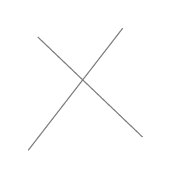
\begin{tikzpicture}[x=1cm,y=1cm]\draw[thin,gray] (0,.15)--(1.2,1.7) (.12,1.59)--(1.45,.32);\end{tikzpicture}}

\diagram{\begin{tikzcd}[ampersand replacement=\&]
 {} \& k\\
 \text{pour}\quad A_1\otimes_k A_2\arrow[ur,"{\mathrm{Tr}_1,\mathrm{Tr}_2}"]\arrow[dr,"\unsure{\text{inc.}|\text{hom.}}", "\text{can.}"'] \& {}\\
 {} \& A_1\otimes A_2
\end{tikzcd}}

\[ E\simeq(E_1\otimes E_2)\oplus(L_1\otimes L_2)\big/(E_1\otimes L_2)+_{L_1\otimes L_2}(\deleted{\unsure{E}}L_1\otimes E_2) \]

\[ A\times E\longrightarrow\underline O\qquad\text{accouplement,} \]

\[
\begin{aligned}
0&\longrightarrow k\longrightarrow A\longrightarrow L_1^\vee\otimes L_2^\vee\longrightarrow0\\
0&\longrightarrow L_1\otimes L_2\mathbin{\unsure{-|\to}}E\longrightarrow\unsure{A|k|\underline O}\longrightarrow0
\end{aligned}
\]

\[
\langle\underset{A_1\otimes A_2}{\overset{}{\underbrace{\deleted{\unsure{x_1\otimes x_2}}f_1\otimes f_2}}},
\underset{L_1\otimes L_2}{\underbrace{\deleted{\unsure{x_1\otimes x_2}}u}}\rangle
=\deleted{\langle\varphi_1(x_1),u_1\rangle\langle\varphi_2(x_2),u_2}
\inserted{\underbrace{\varphi_1(f_1)\varphi_2(f_2)}_{\varphi(x_1\otimes x_2)}.u}
\]

\[
\begin{aligned}
\langle\lambda,x_1\otimes x_2\rangle&=\lambda\psi_1(f_1)\psi_2(f_2)=\lambda\psi(x_1\otimes x_2)\\
\langle\lambda,u\rangle&=0\\
\langle f_1\otimes f_2,x_1\otimes x_2\rangle&
\end{aligned}
\]

\deleted{\unsure{$f_1$}}\quad $x$\quad \deleted{expr. bil. en $\unsure{f_1|f_1\otimes f_2}\langle f_1,x_1\rangle\langle f_2,x_2\rangle$}

\deleted{$f_1\otimes1$}\qquad \deleted{\unsure{vaut sur|nul sur} $\unsure{A}^{\unsure{\leftrightarrows|\natural}}, E^{\leftrightarrows}$}

$(\deleted{A_1\otimes A_2}\ A_1\deleted{\oplus}A_2,$ et sur

Si $f\in A_1$ ou $A_2$, on veut que ce soit $\mathrm{Tr}(f)\psi(x)$

Si $x\in E_1\otimes L_2+L_1\otimes E_2$, \unsure{alors on veut que ce soit|alors on prend} $\varphi(f).\pi(x)$

% archive sheet number: 183
\scanpage{185}
\mspage{496}

le déséquilibre marqué par la valorisation exclusive du yang, auquel il m'est arrivé de faire allusion déjà précédemment (*). La même constatation peut se faire pour la quasi-totalité des couples yin-yang sur lesquels je suis tombé - c'est là une chose vraiment très frappante, que je n'avais jamais pris le loisir précédemment de vérifier de façon aussi circonstanciée.

Parmi les couples écrits tantôt, le seul qui me semble faire exception est le couple p a s s i o n - s e r é n i t é , vu que dans l'usage courant\handwritten{,} le mot ``passion'' souvent s'associe à l'image d'un déchaînement, d'une violence, ou sinon d'un l a i s s e r - a l l e r , avoisinant fâcheusement le nuage d'associations entourant un mot comme `` t u r p i t u d e ''. Comme par hasard, laisser-aller et turpitude désignent des états de déséquilibre psychique caractérisés par une excessive prépondérance y i n , féminine! Et symétriquement, suivant les mêmes mécanismes pousse-bouton (qui révèlent nos conditionnements courants, et nullement la nature d'une chose comme la ``sérénité''), le mot ``sérénité'' s'associe (par opposition à ``passion'') à l'image d'un c o n t r ô l e \ d e \ s o i - d'une qualité donc qui, comme de juste, est d'essence m a s c u l i n e. (En fait, le pendant yin du ``contrôle'' n'est nullement la ``passion'', mais ``l'abandon''.)

Ce qui se passe donc ici, c'est que par suite d'une confusion générale dans les esprits sur la nature de certaines choses, s'exprimant par une égale confusion dans l'usage de certains mots, censés les désigner, il y a une confusion du couple yang-yin ``passion-sérénité'' avec l'ensemble des deux notions
\[ \text{relâchement - contrôle,} \]
dont les termes sont yin-yang (sans pour autant constituer un ``couple'', les deux termes en présence n'ayant aucune envie de s'épouser!). Il me semble donc que la soi-disante ``exception'' à la règle (de la valorisation systématique du yang) en est au contraire une confirmation particulièrement intéressante! Et je ne serais pas étonné qu'il en soit de même avec les autres quelques exemples que j'ai relevés, où dans un couple yang-yin, c'est le terme yin qui semblerait valorisé.

Je ne suis d'ailleurs nullement sûr que cette distorsion dans la vision du monde que je constate dans la civilisation dite ``occidentale'', provenant de ce parti-pris systématique en faveur du masculin, opposé au féminin - que cette distorsion, ce déséquilibre soient tellement moindres dans la tradition chinoise,

\noindent\rule{.22\linewidth}{.4pt}\par
(*) Voir la note ``Yang enterre yin (1) - ou le muscle et la tripe'', n$^\circ$ 106.

% archive sheet number: 184
\scanpage{186}

\diagram{\begin{tikzcd}[ampersand replacement=\&,column sep=small]
1,\arrow[d] \& \deleted{\unsure{x}}u_1,\arrow[d,mapsto] \& u_2,\arrow[d,mapsto] \& u_{\unsure{1|2}}u_{\unsure{2|3}}\arrow[d]\&\sigma_1\sigma_2\\
2 \&\deleted{\unsure{2u_1}}0 \&\deleted{\unsure{2u_2}}0 \& 2u_1u_2=v\&{}
\end{tikzcd}}

\[ v\longmapsto 2u_{\unsure{2|1}}u_3 \]

\[1\quad -u_1^2=c_1 1,\ -u_2^2=c_2.1,\quad u_1^2u_2^2=c_1c_2 \]

\diagram{\begin{tikzcd}[ampersand replacement=\&,column sep=small,row sep=huge]
 E_1\otimes E_2\arrow[rr]\arrow[rrr,bend left=25,"{x_1\otimes x_2\longmapsto x_1\otimes x_2+\overline{x}_1\otimes\overline{x}_2}"] \& {} \& E_1\wedge E_2\arrow[r,"?"] \& E_1\otimes E_2\\
 E_1\otimes_0 E_2\arrow[u,"\unsure{\text{inc.}|\text{hom.}|\text{can}}"]\arrow[r,"\pi"'] \& L_1\otimes L_2\arrow[ur]\arrow[urr,"{u_1\otimes u_2\longmapsto u_1\otimes u_2}"']\arrow[rr,"{\text{i.e. }\unsure{\text{comm.}}}","\mathrm{id}"'] \& {} \& L_1\otimes L_2\arrow[u,hook,"\text{can}"]
\end{tikzcd}}

\[ \deleted{\unsure{E_2}}\quad\begin{matrix} E_1\otimes L_2\\ \rotatebox{90}{$\in$}\\x_1\otimes u_2\end{matrix} \]

\[
\begin{aligned}
\pi_1(x_1)\otimes u_2&=(2x_1-\inserted{\psi_1(x_1)}T_1)\otimes u_2\\
x_1\otimes u_2&+(\psi_1(x_1)T_1-x_1)\otimes(-u_2)\\
&=2x_1\otimes u_2-\psi_1(x_1)T_1\otimes u_2
\end{aligned}
\]

\margin{OK}

\[
\begin{aligned}
(x_1+u_1)*(x_2+u_2)&=(\sigma+\overline{\sigma})[(x_1+u_1)\otimes(x_2+u_2)]\\
&=x_1*x_2+\pi_1(x_1)\otimes u_2+u_{\unsure{1|2}}\otimes\pi_2(x_2)+\underbrace{u_1*u_2}_{=\,2u_1\otimes u_2}\\
&\hspace{4em}b_1\otimes u_2+u_2\otimes b_{\unsure{3|1|2}}+2u_1\otimes u_2
\end{aligned}
\]

\[ \deleted{b_1u_2+b_2u_1+u_1} \]

\diagram{\begin{tikzcd}[ampersand replacement=\&,column sep=small,row sep=small]
 (x_1+u_1)\unsure{\circ|*}(x_2+u_2)= \& x_1\unsure{*|\circ}x_2\arrow[d,mapsto] \& {}+\big(\underbrace{b_1u_2+b_2u_1+2u_1u_2}\big) \& {}\in E_1\wedge E_2\arrow[d]\\
 {} \& x_1*'x_2\arrow[d,equal] \& {} \& E_1\otimes E_2\\
 {} \& \mathrm{Tr}_{E_1\otimes E_2/E_1\wedge E_2}(x_1\otimes x_2) \& {} \& {}
\end{tikzcd}}

% archive sheet number: 185
\scanpage{187}
\mspage{500}

tant bien que mal. Cette réalité ``sociale'' est le produit d'un conditionnement immémorial, lequel très tôt prend racine dans le ``moi'' en formation et le structure. Pourtant, au delà de cette réalité-là, il est une réalité plus profonde, venant de beaucoup plus loin encore, laquelle est déterminante dans la pulsion amoureuse elle-même. C'est la réalité d'une c o m p l é m e n t a r i t é profonde, essentielle des sexes, où il n'y a nulle place pour un quelconque ``antagonisme''. C'est la réalité aussi qui se manifeste clairement dans toutes les espèces vivantes, à la seule exception de la nôtre, où elle se trouve occultée dans une large mesure par l'antagonisme culturel, donc par un état de d i v i s i o n propre à l'homme et à la société humaine.

Les clichés courants romantiques, style ``Nous Deux'', qui dominent une grande partie de la littérature et des médias, montent d'ailleurs en épingle une ``complémentarité'' de pacotille, tout en jetant un voile pudique sur le troublant aspect antagoni\handwritten{s}te homme-femme, ou (au mieux) en le traitant comme une sorte d'accident un peu piquant, bienvenu pour mettre quelque piment dans un repas un peu trop fadasse\unsure{.} ou sirupeux sinon. Dès qu'on dépasse ce gen\handwritten{re de} clichés rassurants, on se voit aussitôt confronté à la réalité de cet antagonisme homme-femme - réalité apparemment universelle, et au surplus d'une tenacité à toute épreuve, une tenacité de chiendent! Mais \hspace{.6em}partir de cette réalité omniprésente et irrécusable, pour instituer une sorte d'antagonisme cosmique du yin et du yang, du ``féminin'' et du ``masculin'', c'est projeter sur l'Univers entier l'état de déchirement, de division profonde de la société humaine et de la personne, une maladie donc propre à notre espèce. C'est aussi perpétuer sa propre ignorance d'une a u t r e réalité en soi-même (rejoignant cette réalité cosmique de l'harmonie des complémentaires), d'une réalité toute aussi tenace (ou, pour mieux dire, indestructible), mais plus cachée. Cette réalité va à l'encontre des conditionnements instituant tacitement un antagonisme de fait aussi bien entre la femme et l'homme, l'épouse et l'époux, qu'entre cela en nous-même qui est ``femme'' et ce qui est ``homme''.

A vrai dire, cette vision d u a l i s t e ou g u e r r i è r e de l'Univers, où un aspect des choses se trouverait en guerre constante avec un aspect ``symétrique'' tout aussi essentiel - cette vision n'est nullement le fruit d'une r é f l e x i o n , qui ``partirait'' (comme j'écrivais à l'instant) de la réalité du conflit dans le couple humain et dans la société humaine, pour la ``déduire'' ensuite (ou ``l'instituer'', comme j'écrivais plus justement) dans le Cosmos tout entier. Elle n'est ni plus, ni moins que l'expression fidéle, automatique autant dire, du conditionnement culturel, et va dans le sens d'une

% archive sheet number: 186
\scanpage{188}

Considérons $\langle u_1*u_2,x_1*x_2\rangle={}$

\[ \deleted{x_1*x_2} \]

\diagram{\begin{tikzcd}[ampersand replacement=\&]
 {} \& A_1\otimes A_2\oplus(A_1\oplus_{O}A_2)\arrow[d]\\
 A_1\otimes A_2\arrow[ur] \& A
\end{tikzcd}}

\diagram{\begin{tikzcd}[ampersand replacement=\&,column sep=small]
 A_1\otimes A_2\arrow[r,"\unsure{\text{inj}|\text{can}}"] \& (A_1\otimes A_2)\oplus(A_1\oplus_{\underline O}A_2)\arrow[r,"\unsure{\text{quot}|\text{proj}|\text{surj}|\text{somme}}"] \& A\\
 {} \& \deleted{E_1\otimes E_2\longrightarrow}\arrow[r,no head] \& E
\end{tikzcd}}

\[ \deleted{A=A_1\otimes A_2\times\underline O\oplus(\unsure{A_1+A_2})}\big/\mathrm{Im}\,(A_1\oplus_{k}A_2) \]

\deleted{$\deleted{E}A^\vee\simeq{}$ Formes bilin. sur $\deleted{\unsure{E_1\times E_2}}A_1\times A_2$ telles que}

\[
A^\vee\simeq(f,\deleted{\unsure{g_1,g_2}}\inserted{\lambda})\quad\text{avec}\quad
\left\{\begin{aligned}
& f\ \text{forme bil. }\deleted{\text{sur}}\ A_1\times A_2\longrightarrow k\\
&\deleted{g_1:\unsure{g}A_1\longrightarrow k}\qquad\lambda\in k\\
&\deleted{g_2:A_2\longrightarrow k}
\end{aligned}\right.
\]

satisfaisant \deleted{\unsure{la relation}}

\deleted{a) $g_1(1)=g_2(1)$ i.e. $g$ provient d'une} forme sur

\diagram{\begin{tikzcd}[ampersand replacement=\&,column sep=small] A_1+A_2\arrow[dr,bend right=28] \& {}\subset A_1\otimes A_2\\ {} \& k \end{tikzcd}}

\[
\begin{aligned}
 &\deleted{\text{b) } f\mid(A_1+A_2)=\underline{\underline{2}}g\quad\text{i.e.}}\\
 &\deleted{f(x_1,1)=2g_1}\\
 &\deleted{f(\unsure{1|x_1},x_2)=2g_2}
\end{aligned}
\]

\[
\begin{aligned}
f(x_1)&=\lambda\mathrm{Tr}_1(x_1) &u_1&\in A_1\\
f(x_2)&=\lambda\mathrm{Tr}_2(x_2) &u_2&\in A_2
\end{aligned}
\]

\diagram{\begin{tikzcd}[ampersand replacement=\&,column sep=small,row sep=small]
 \unsure{0|\cdot}\arrow[r] \& L_1\otimes L_2\arrow[r,no head] \& E\arrow[r,"\psi"] \& O\arrow[r] \& 0\\
 \deleted{E\longrightarrow A^\vee\unsure{?}}\&{} \& \underset{x}{\rotatebox{90}{$\in$}} \& E \& {}\\
 {} \& \deleted{\lambda=\unsure{\varphi(x)}} \& {} \& {} \& {}
\end{tikzcd}}

% archive sheet number: 187
\scanpage{189}
\mspage{497}

\texttt{ou même dans le monde chinois (ou plus généralement le monde ``oriental'') d'aujourd'hui. Aucun signe, au niveau de la vie de tous les jours, ne pourrait me le} faire supposer, ni à travers mes amis et amies orientaux, ni à travers les échos qui ont pu me parvenir de la tradition et de la vie \handwritten{d'} aujourd'hui dans la Chine ou d'autres pays d'extrême-Orient - bien au contraire. Il me semble plutôt qu'une fine perception du dynamisme yin-yang s'est cantonnée à peu près exclusivement dans la p r a t i q u e de c e r t a i n s \ a r t s - comme la calligraphie, la poésie, l'art culinaire et, bien entendu, l'art médical (*).

C'est le dernier surtout, sous le nom de ``médecine chinoise'' et par le biais de certains succés spectaculaires de l'acupuncture, qui a fini au cours de\unsure{s} vingt ans passés, par acquérir droit de cité chez nous, et à être investi de prestige. Nombreux pourtant sont encore ceux qui ignorent qu'en médecine chinoise, l'alpha et l'oméga de l'appréhension du corps, de la circulation d'énergie dans le corps et des perturbations de celle-ci (qui constituent les états morbides que nous appelons ``maladies''), se trouve justement dans une dialectique très fine du yin et du yang. Le fait que cette dialectique ``marche'', puisque la ``médecine chinoise'' basée sur elle est efficace (y compris dans de nombreux cas qui échappent aux moyens de la panoplie occidentale), peut être considéré comme une sorte de ``preuve'' de la réalité des ``principes'' ou `` aspects'' ou ``modes'' (d'appréhension, ou d'exist\handwritten{e}nce) yin et yang - que ce ne sont pas de pures spéculations sorties des chapeaux de certains philosophes et autres poètes (pour ne pas dire fumistes).

On peut se demander, il est vrai, quel est le sens de telles preuves, et même de toute ``preuve'' quelle qu'elle soit de la validité de telle ou telle vision du monde. A supposer même que la preuve ait convaincu (c'est-à-dire, que l'intéressé ait bien voulu se laisser convaincre), et même et par dessus le marché\handwritten{,}que la vision en question soit profonde et par là,bienfaisante - la meilleure preuve du monde est impuissante pourtant à c o m m u n i q u e r

\noindent\rule{.22\linewidth}{.4pt}\par
(*) (21 octobre) J'ai oublié dans le nombre l' a r t \ d i v i n a t o i r e , dans le Y i \ K i n g ou ``livre des changes'', qui jouit aujourd'hui d'une\unsure{.} grande popularité dans certains milieux tant en Europe qu'en Amérique. Les 64 ``hexagrammes'' qui constituent les ``mots'' de base du langage divinatoire du Yi King, ne so\unsure{nt} autres que les $2^{\handwritten{6}}$ combinaisons possibles de suites de six ``signes'' yin et yang, depuis le yin pur (six répétitions du yin ) au yang pur (six répétitions du yang\unsure{).} Il semble y avoir là une sorte d'alchimie d'une grande finesse des combinaisons du yin et du yang, qui\handwritten{(}paraît-il\handwritten{)} avait fasciné Jung. L'intérêt de cette alchimie \handwritten{(}en tant que``collection d'archétypes'' notamment) me paraît a priori indépendant de son usage en art divinatoire, et du crédit qu'on est disposé à accorder à un tel usage.

% archive sheet number: 188
\scanpage{190}

\deleted{\unsure{Le}} $u$ divalent en termes des $u_1,u_2$ ?

\deleted{\unsure{$u=2u_1$|$u=u_1$} \unsure{comparer|Comparons}}

\deleted{Comment \unsure{calculer|Considérons}} On doit avoir

\[ u_1\overset{\unsure{s|\xi}}{*}u_2=\underline{\lambda}u+\underline{\mu}\qquad\text{trouver }\lambda,\mu \]

\[
\begin{aligned}
 \mathrm{Tr}_{A/k}^{\unsure{c}}(u_1*u_2)&=-\deleted{\unsure{2}}\lambda\beta+2\mu\\
 N_{A/k}(u_1*u_2)&=\underline{\lambda^2}c+\underline{\mu^2}\deleted{\unsure{+}}\unsure{-}\underline{\lambda\mu}\beta
\end{aligned}
\]

\[ \deleted{\mathrm{Tr}_{A_1\otimes A_2}} \]

\[
\begin{aligned}
&\text{base de }A &&1,u\\
&\text{base \inserted{duale} de }E &&
\deleted{e=e_1\otimes e_2,\ x=x_1*x_2}\\
&&&x=x_1*x_2,\ e=e_1\otimes e_2.
\end{aligned}
\]

\[
\begin{aligned}
\langle1,x\rangle&=1 &\langle1,\unsure{x|e}\rangle&=0\\
\langle{u},e\rangle&=1 &\langle u,x\rangle&=0
\end{aligned}
\]

\[
\begin{aligned}
\lambda&=\deleted{\langle u,e\rangle}\langle u_1*u_2,\overbrace{e_1\otimes e_2}^{e}\rangle\\
\mu&=\langle u_1*u_2,\underbrace{x_1*x_2}_{x}\rangle
\end{aligned}
\]

\[ u_1*u_2 \]

\[ \mathbb F_2\longrightarrow\mathbb F_2\times\mathbb F_{\unsure{2|1}} \]

\diagram{\begin{tikzcd}[ampersand replacement=\&,column sep=large,row sep=small]
 \deleted{\unsure{E}}A_1\otimes A_2\arrow[r,"*"]\arrow[rr,bend left=22,"\deleted{\unsure{x_1\otimes x_2}}"]\arrow[d,phantom,"\times"] \& A\arrow[r,"\unsure{\leftrightarrows|\natural|\xi}"{draw,circle},"{(\unsure{\sigma|\mathrm{I}|\mathrm{Tr}})}" description]\arrow[d,phantom,"\times"] \& A_1\otimes A_2\arrow[d,phantom,"\wedge"]\\
 E_1\otimes E_2\arrow[d] \& E\arrow[l,"\leftrightarrows"']\arrow[d] \& \deleted{A}E_1\otimes E_2\arrow[l,"*"{draw,circle,swap}]\arrow[d]\\
 \underline O \& O \& \underline O
\end{tikzcd}}

\[
\begin{aligned}
&\deleted{(x,y)\longmapsto \unsure{x\otimes y,\ x+}}\\
&{}^t(\mathrm{id}+\deleted{\unsure{\mathrm{id}}}\sigma_1\otimes\sigma_2)
=\mathrm{id}+\underset{=\sigma_1}{({}^t\sigma_1)}\otimes\underset{=\sigma_2}{{}^t(\sigma_2)}
\end{aligned}
\]

\deleted{\unsure{$x_1$}}\qquad\deleted{$u_1\otimes u_2$}

\[
u\in A\qquad\text{défini par}\quad
\left\{\begin{aligned}
\langle u,e_1\otimes e_1\rangle&=1\\
\langle u,x_1*x_{\unsure{2|1}}\rangle&=0
\end{aligned}\right.
\]

% archive sheet number: 189
\scanpage{191}
\mspage{498}

u n e \ v i s i o n , et encore moins une vision du monde. Cela vous fait une belle jambe d'être ``convaincu'' mordicus d'une vision qui reste étrangère, incomprise. Pour tout dire, cela n'a pas même de sens - ou plus exactement, le vrai sens de sa ``conviction'' n'est pas plus compris par l'intéressé, que cette vision qu'il fait mine d'incorporer à son lourd bagage culturel.

Quand la vision est comprise et assimilée, la question même d'une ``preuve'' apparaît étrangement saugrenue - un peu comme de prouver que le ciel est bleu quand on voit bien qu'il est bleu, ou que le parfum d'une fleur qu'on aime est bon...

\figure{\begin{tikzpicture}\draw[gray,thin] (0,0).. controls (-.06,.30) and (.12,.68)..(.47,1.04);\end{tikzpicture}}

(\textsuperscript{112}) (17 octobre) Mes premières réflexions sur le double aspect ``féminin'' et ``masculin'' sont issues d'une réflexion sur moi-même. C'était vers les débuts 1979, à un moment où j'ignorais encore les mots chinois ``yin'' et ``yang'', et l'existence d'une sorte de ``philosophie'' subtile du jeu incessant du yin et du yang, dans la tradition culturelle chinoise. J'ai appris la chose vers la fin de la même année je crois, par ma fille et surtout par mon gendre Ahmed, qui commençait alors à s'intéresser à la médecine chinoise, sur laquelle il a accroché fortement dans les années suivantes. La plupart de ce qu'il me disait recoupait et confirmait la vision à laquelle j'étais parvenu, chose qui n'avait rien pour me surprendre. Si surprise il y avait, c'était plutôt dans les quelques cas de ``couples'' où le rôle yin-yang ``naturel'' me semblait renversé, dans la tradition chinoise. Mon réflexe (fortement ``yang'' en l'occurence!) avait été une conviction à fleur de peau que ce ``renversement'' devait être dû à une déformation culturelle, sans d'ailleurs aller y regarder de trop près (*) - c'étai\unsure{t} à un moment où mes gammes passées sur le féminin-masculin me paraissaient bien lointaines, alors que j'étais engagé dans une méditation autrement plus personel\unsure{-}

\noindent\rule{.22\linewidth}{.4pt}\par
(*) Cette réaction d'assurance péremptoire, vis-à-vis d'une tradition millénaire qui aurait pu m'inciter à plus de prudence, est celle-là même qui, enfant, m'a fait récuser la formule (bien compliquée ma foi!) $\handwritten{\pi}=3{,}14\ldots$ enseignée par les livres, en faveur de $\handwritten{\pi}=3$ dont je m'étais convaincu par mes propres moyens. (Voir la note ``La quadrature du cercle'', n$^\circ$ 69.) Il est vrai que pour cette histoire du yin et du yang, j'avais eu ample occasion de me rendre compte à quel point l'appréhension de la nature du ``féminin'' et du ``masculin'', et de leurs interrelations, est faussée par des distortions culturelles invétérées, d'une force considérable. Je ne me rendais pas compte encore, par contre, à quel point aussi une appréhension précise et délicate de ces relations était chose essentie\unsure{l}le dans la pratique de certains arts traditionnels chinois, et poussé à un degré de grande finesse.

% archive sheet number: 190
\scanpage{192}

\[
\begin{aligned}
u_1&\quad u_1^2+b_1 x_1+c_1=0\\
u_2&\quad u_2^2+b_2x_2+c_2=0
\end{aligned}
\]

\[ u_1*u_2=u_1\otimes u_2+(u_1+b_1)\otimes(u_2+b_2)=2u_1u_2+b_2u_1+b_1u_2+\underline{\underline{b_1b_2}} \]

\unsure{ne forme} \unsure{enti.} \deleted{\unsure{n'est pas déf. une}} une base de $A$ avec $1$ \unsure{S'annule|s'annule} si $2=0$, $b_1=b_2=0$

\[
\begin{aligned}
A_1&\simeq\deleted{\unsure{L_1}}\underline O\oplus\deleted{\unsure{O}}L_1^\vee &
 A_2&=\deleted{\unsure{L_2}}O_{\unsure{2}}\oplus L_2^\vee\\
E_1&\simeq O+L_1, & E_2&\simeq\underline O+L_2
\end{aligned}
\]

\[
\begin{aligned}
&\deleted{A\simeq L_1^\vee\otimes L_2^\vee+}\\
&A\simeq\underline O\unsure{\oplus|\otimes} L_1^\vee\otimes L_2^\vee
\end{aligned}
\]

\diagram{\begin{tikzcd}[ampersand replacement=\&,column sep=small,row sep=small]
 E_1\otimes E_2\arrow[r,no head]\&E_1\wedge E_2\arrow[r]\&E_1\otimes E_2\\
 x_1\otimes x_2\&x_1\deleted{\unsure{\otimes}}*x_2\&\mathrm{Tr}_{\unsure{1|,}}(x_1\otimes x_2)
\end{tikzcd}}

\[
\begin{aligned}
e_1&\in L_1 & e_2&\in L_2\\
&\text{base de }L_1 &&\text{base de }\unsure{e_2|L_2}
\end{aligned}
\]

\[
\begin{aligned}
\unsure{x_1}\qquad b_1&=\beta_1e_1 &c_1&=\gamma_1e_{\unsure{2|1}}^{\unsure{\otimes2|\otimes}}\\
b_2&=\beta_2e_2 &c_2&=\gamma_2 e_2^{\otimes2}
\end{aligned}
\]

\[
\begin{aligned}
 A&\simeq\underline O+\unsure{k|O}\deleted{\unsure{x}}e_1^* &
 u_1&=e_1^*\\
 &&u_2&=e_2^{\unsure{*|\circ}}
\end{aligned}
\]

\[
\begin{aligned}
\deleted{u_1^2+\beta_1u_1=\unsure{e_1^*}}&\quad u_1^2+\beta_1u_1+\gamma_1=0\\
\deleted{\unsure{u_1^2+(\beta_1 e_1)u_1}}&\quad u_2^2+\beta_{\unsure{1|2}}u_2+\gamma_2=0\\
&u=\unsure{2uu'}+
\end{aligned}
\]

\[
\begin{aligned}
 x_1,e_1&\longleftrightarrow u_1\in A_1 \qquad u_1^2+\beta_1u_1+\gamma_1=0\\
 \deleted{\unsure{x,e_1}}&\qquad
 \left\{\begin{aligned}
 e_1&=\varphi(u_1)\\
 \langle\unsure{u_1|x_1}\deleted{\unsure{+}},x_1\rangle&=0\\
 \unsure{\varphi|\psi}(x_1)&=1
 \end{aligned}\right.
\end{aligned}
\]

\[
\begin{aligned}
(x_2,e_2)&\longleftarrow u_2\in A_2\ \big|\ u_2^2+\beta_2u_2+\gamma_2=0\\
(x_1*x_2,e_1\otimes e_2)&\longleftrightarrow u\in A.\\
&\hspace{4em}u^2+\beta u+\gamma=0
\end{aligned}
\]

% archive sheet number: 191
\scanpage{193}
\mspage{499}

le sur la vie de mes parents et sur mon enfance. C'est des mois ou des années pl\unsure{us} tard seulement, je crois, que par un certain nombre de recoupements, je me suis rendu compte que dans certains cas mon appréhension des rôles yin et yang dans tels ou tels ``couples'' était resté un tantinet superficielle; que j'avais mis da\unsure{ns} le même sac, un peu hâtivement, des situations de nature différente que la diale\unsure{c}tique yin-yang chinoise prenait bien soin de distinguer (112\handwritten{$'$}). Maintenant, je m\unsure{e} rends compte que l'appréhension du yin et du yang reste encore relativement grossière et statique chez moi, surtout si on la compare à la finesse requise pour l'exercice de certains arts traditionnels chinois comme la médecine (intimement liée aussi à la diététique et à l'art culinaire), où cette appréhension finit pa\unsure{r} devenir comme une seconde nature.

J'ai eu l'impression plus d'une fois que chez les pratiquants et praticiens de ces arts, qu'ils soient orientaux ou européens, cette finesse d'appréhension reste fragmentaire, en ce sens qu'elle reste, dans une très large mesure, soigneusement cantonnée dans l'exercice de cet art. Dans la vie de tous les jours, elle agirait plutôt comme un ``savoir'' ordinaire, se superposant purement et simplement au ``savoir'' du conditionnement culturel (et autre), et restant plus ou moins lettre morte vis-à-vis de celui-ci. Pour le dire autrement, j'ai eu l'impression que la vision du monde et de soi, et les mécanismes de répression dans la perception de la réalité, ne sont en rien différents chez ces personnes tout ce qu'il y a d'``averties'', que chez le commun des mortels.

Cette impression se recoupe avec une autre, que j'ai eue en parcourant deux ou trois textes, écrits par des européens censés être ``dans le coup'', qui se proposent de donner un aperçu de la philosophie traditionelle chinoise du yin et du yang. (L'un des auteurs est un orientaliste français bien connu, dont le nom m'échappe à présent.) La chose qui m'a frappée, c'est que dans ces textes, le yin et le yang sont présentés comme des principes ``o p p o s é s'' (ou ``c o n t r a i r e s'') voire a n t a g o n i s t e s (ce dernier terme revient à plusieurs reprises dans un de ces textes), plutôt que c o m p l é m e n t a i r e s. Cette ``opposition'' ou ``antagonime'' aurait son expression typique dans celui qui aurait lieu entre la femme et l'homme à l'intérieur de la société humaine, et à l'intérieur du couple institué par la société.

L'antagonisme dans le couple époux-épouse est bel et bien une réalité, aussi bien à l'Est qu'à l'Ouest. Elle est profondément enracinée dans la culture, à tel point qu'il peut paraître parfois comme un des aspects (parfois déroutant!) de la condition humaine, voire même comme la racine du conflit en l'homme ou dans la société humaine. La réalité de cet antagonisme est irrécusable, et elle dépasse certes les clichés courants qui s'efforcent de l'exorciser

% archive sheet number: 192
